\section{Introduction}
As development of robotic technology, more and more people expect intelligent robots to serve the family as human beings and provide a good and comfortable life experience. The RoboCup@Home competition \cite{robocupathome} focus on bringing robotics to apply in common domestic environment. To achieve such goal, the robotic system must be able to perceive environment, communicate with humans and complete various tasks, such as cleaning up a table, holding a party or guiding new comers. Security is the top priority. Because service robots can't do harm to people and the environment. Secondly, the robot should be controllable. The operator can intervene the behavior of the robot at any time to prevent the unexpected situation. Finally, the robot should have complete autonomous action ability and give people comfortable interaction experience. 

The Robotics and Artificial Intelligence Lab (RAIL) of tongji university was founded in 1992, Team TJArk of RAIL was founded in 2004 and participated in RoboCup World Cup from 2006 to 2018. We have got seven winning streak in China RoboCup SPL and once won the third place in RoboCup2018 SPL.
In December 2018, we founded an energetic new team to participate in RoboCup @Home League, called TJArk@Home. Main goal of TJArk@Home is to explore the limit of how well can robots serve people during common life with acceptable cost. Under the guidance of such wish, we are doing many research on the Pepper platform, such as
\begin{itemize}
\item SLAM(Simultaneous Localizaiton and Mapping)
\item Auto navigation of robot
\item Object Detection and Recognition
\item Human-face detection and analysis
\item Human-Robot interaction
\item Motion control
\item Trajectory teaching
\item Design of laptop GUI
\item ...
\end{itemize}
April 2019,  the first time TJArk@Home involved in China RoboCup@Home League, we got the first-place in SSPL(Social Standard Platform League). 
During the competion, we show a lot of abilities, including 
Autonomous navigation, 
Follow an operator to the given position, 
Recognize speech and response, 
Detect humans in vision and summarize their features.
\begin{figure}[!h]

    \centering
    \subfigure[Team photo at China RoboCup 2019]{\label{fig:pepper1}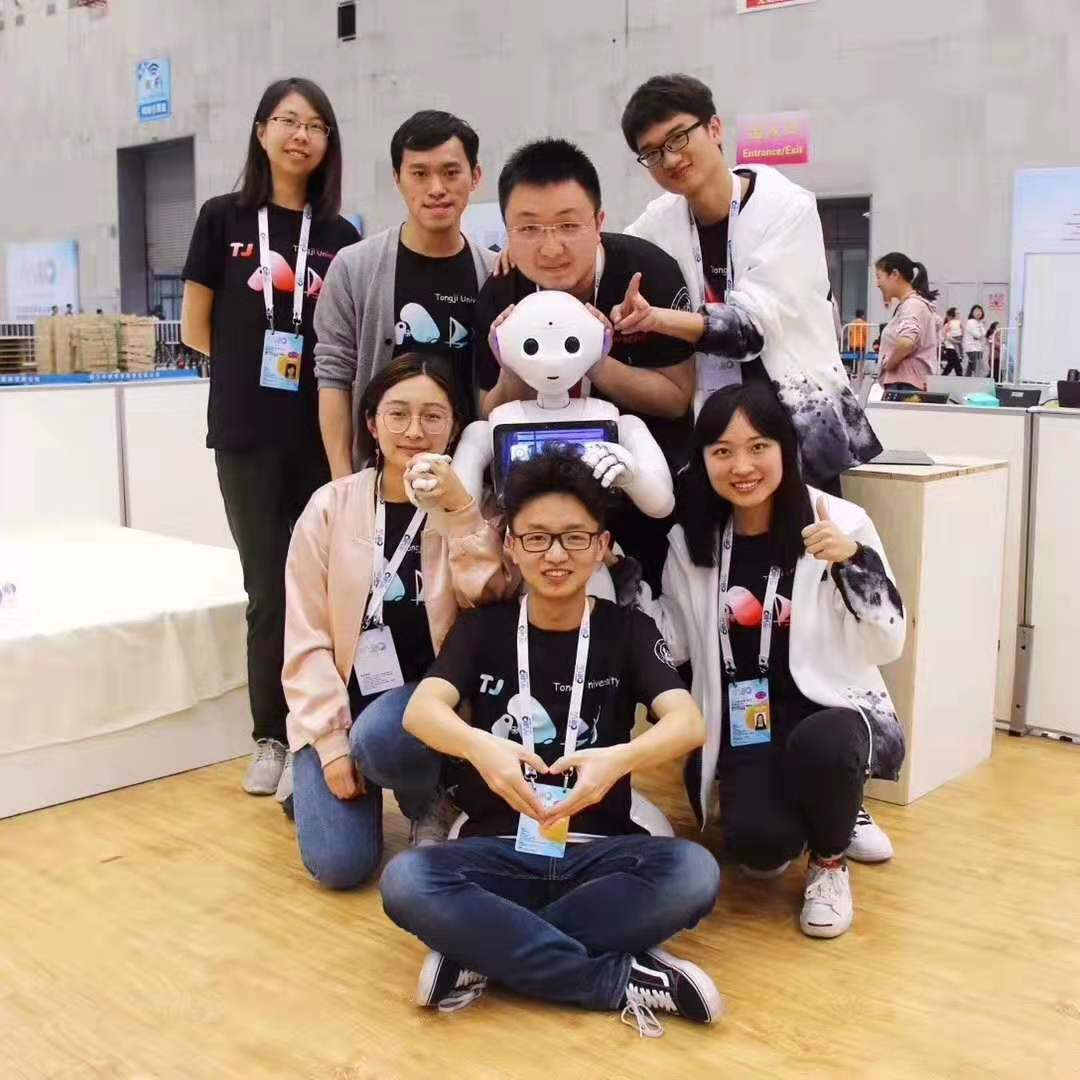
\includegraphics[height=2.5in]{figs/pepper1.jpg}}
    \hspace{0.2in}
    \subfigure[Pepper in homemade scenario]{\label{fig:pepper2}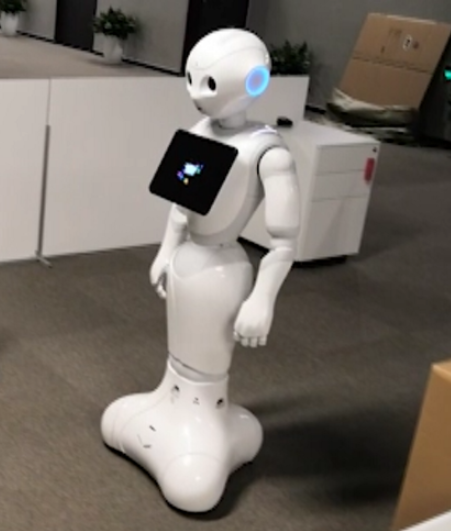
\includegraphics[height=2.5in]{figs/pepper2.png}}
    \caption{Our Pepper}
\end{figure}
Although our team has not been established for a long time, we have developed a reusable and extensible software framework. 
It is a higher level integration of NAOqi API, which makes developing a new application more easily. 
ROS-based components with a bridge to NAOqi are also developed. 
The HTTP-based Information Exchange System(HIES) also helps a lot. 
Tasks require large computational resources such as syntactic analysis can be allocated to a host server. 
Pepper just need seed raw data and listen for response. Such mechanism reduce Pepper’s burden, allowing it pay more attention to interaction logic and task excution. 

Tongji RAIL lab has been researching on robotics since its begining, and achieved a lot in several aspects, such as humanoid walking \cite{rebalancecontrol,CPG}, object detection \cite{FocalLoss}, fuzzy systems \cite{Zhang2018A}. 
RoboCup@Home League is a new attempt, which involves some former research, but bringing untouched challenges like human-robot interaction. 
We are pushing researchs on vision, navigation, interaction and building a simulated competition scenario for integration testing.
